\documentclass[10pt]{article}

\usepackage[utf8]{inputenc}
\usepackage[T2A]{fontenc}
\usepackage[russian, english]{babel}

\usepackage{amssymb, amsmath, textcomp, tabularx, graphicx}
\usepackage{indentfirst}

\title{Отчет по заданию 1}
\author{Андрей Коновалов, 073}
\date{}

\begin{document}

\maketitle

\section{Постановка задачи}

Трубется сравнить критерий Фишера и WM-критерий для решения задачи:
\begin{align*}
    & X_1^n: X_{1i} \sim N(\mu_1, \sigma_1^2), \; X_2^n: X_{2i} \sim N(\mu_2, \sigma_2^2) \\
    & H_0: D X_{1i} = D X_{2i} \\
    & H_1: D X_{1i} \neq D X_{2i} \\
    & \mu_1 = 0, \sigma_1 = 1, \mu_2 = 0 \\
    & \sigma_2 = 0.5 : 0.01 : 2.0, n = 5 : 1 : 50
\end{align*}

\section{Результаты}

Однократная генерация выборок дает результаты изображенные на рис. 1 и 2.
Получившиеся результаты достаточно нестабильные; они не позволяют точно оценить границы области, где нулевая гипотеза отклоняется.
Сделаем усреднение по большому числу экспериментов.

Результаты усреднения по 1000 выборок изображены на рис. 3-6.
Графики оценок мощностей критериев, как и ожидалось, выглядят очень похоже на инвертированные графики p-value.

Из графиков видно, что при увеличении объема выборки отличие дисперсий распределений оказывает большую роль на значение p-value.
Кроме того, WM-критерий принимает гипотезу при большей разности дисперсий, чем критерий Фишера.
При малом размере выборки оба критерия принимают гипотезу при любом значении дисперсии из рассмотренных.
При большом размере выборки критерий Фишера отвергает гипотезу при отклонении дисперсии более, чем на 0.3, а WM-критерий - более, чем на 0.45.

На рис. 7 и 8 изображены зависимости разности достигаемых уровней значимости и мощностей критериев от параметров.
По графикам видно, что достигаемый уровень значимости критерия Фишера почти всегда ниже, чем у WM-критерия, а оценка мощности - выше.

В целом, по графикам, критерий Фишера выглядит более точным.

\begin{figure}[h]
  \centering
  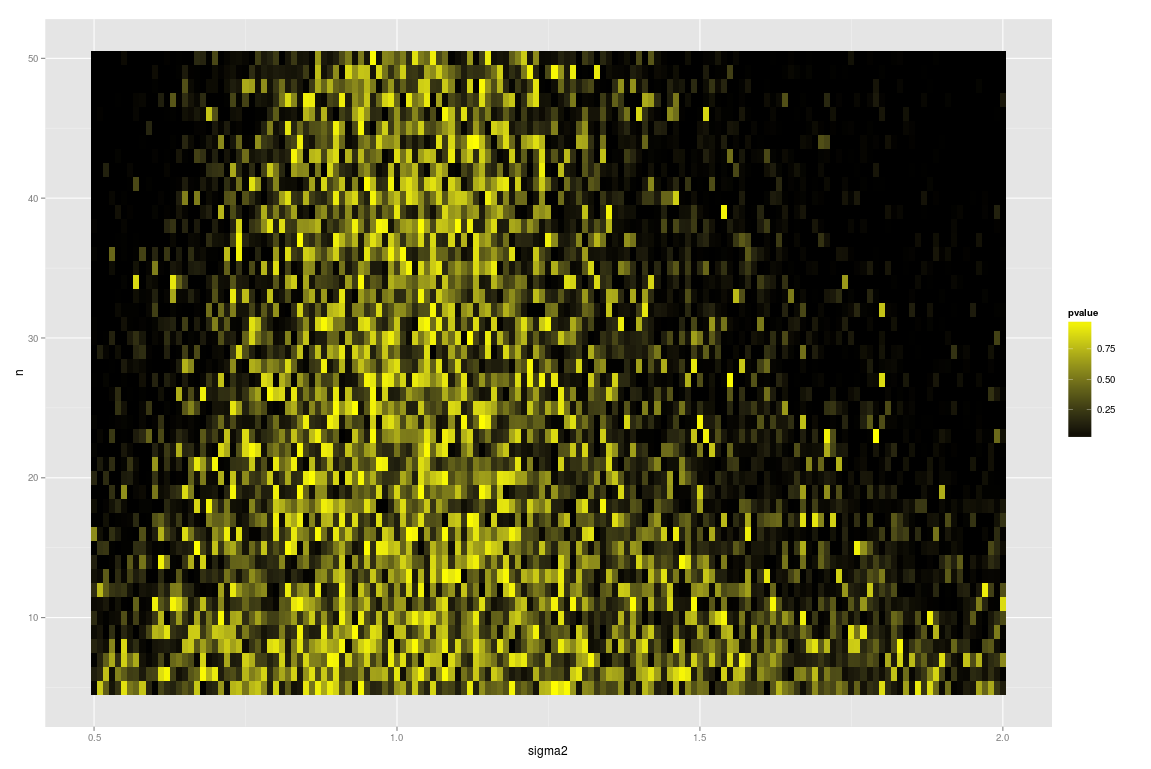
\includegraphics[width=300pt]{f_pvalue_1.png}
  \caption{Зависимость достигаемого уровня значимости от значений параметров при однократном проведении эксперимента для критерия Фишера.}
\end{figure}

\begin{figure}[h]
  \centering
  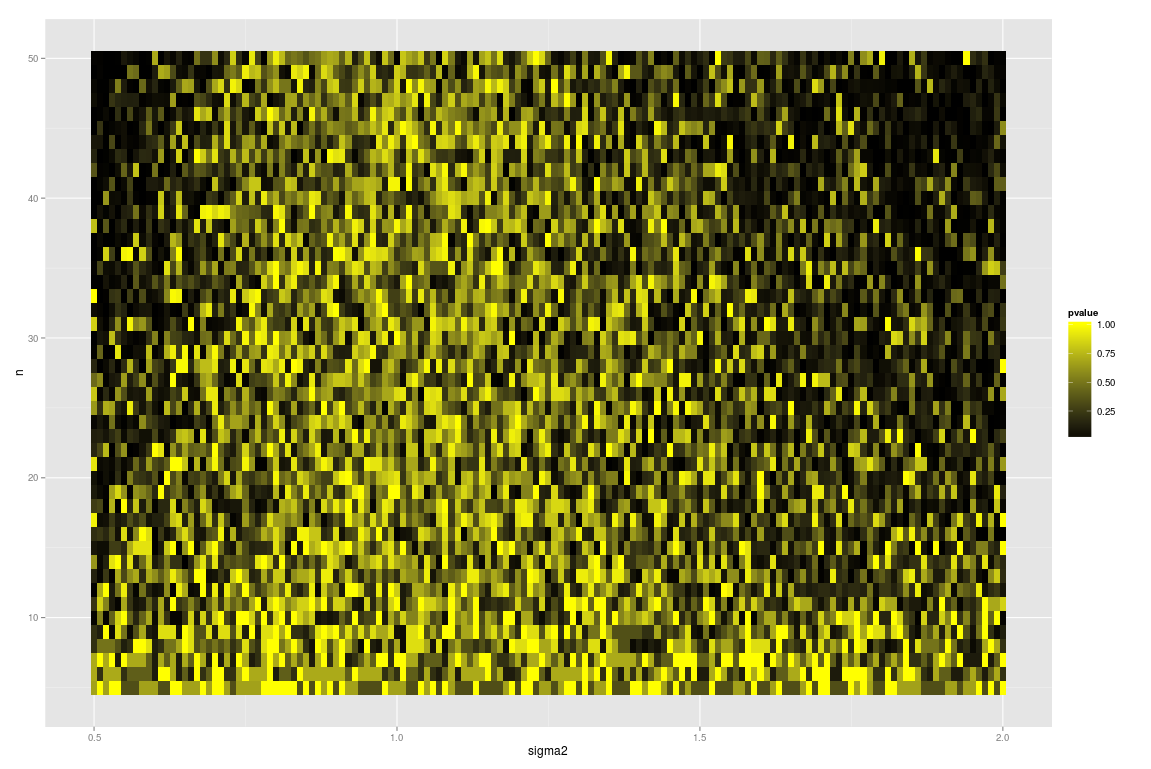
\includegraphics[width=300pt]{wm_pvalue_1.png}
  \caption{Зависимость достигаемого уровня значимости от значений параметров при однократном проведении эксперимента для WM-критерия.}
\end{figure}

\begin{figure}[h]
  \centering
  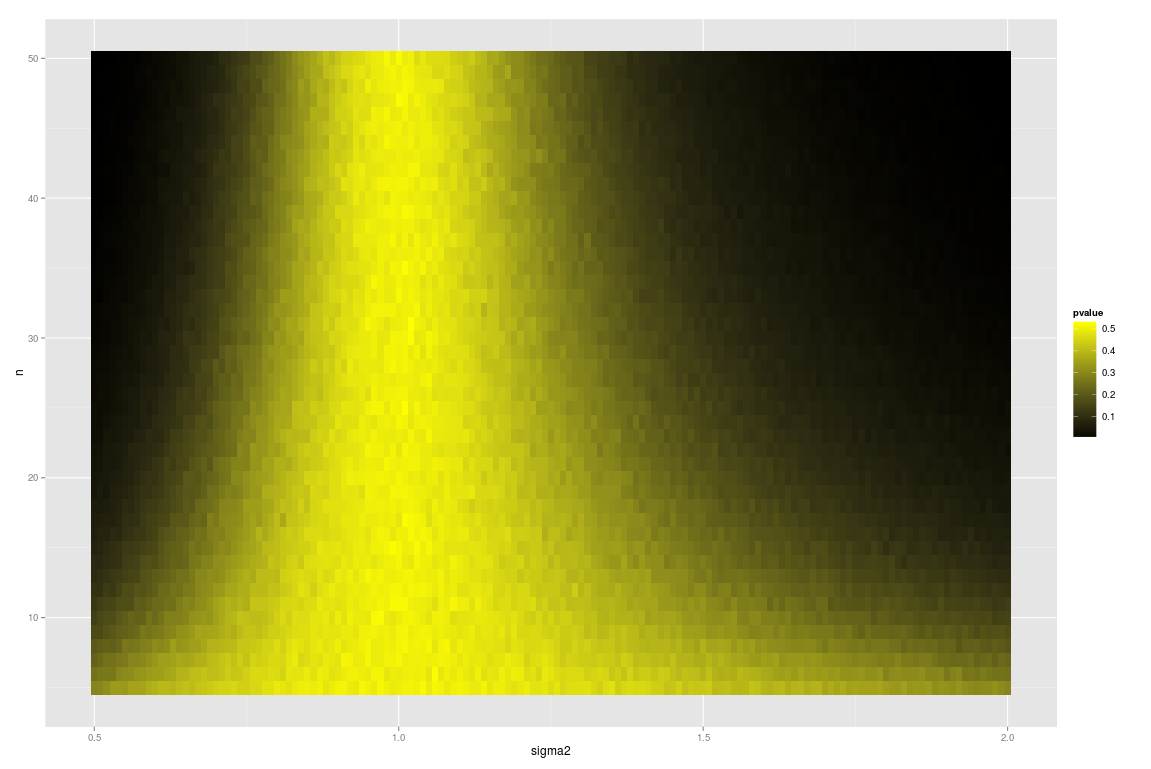
\includegraphics[width=300pt]{f_pvalue.png}
  \caption{Зависимость достигаемого уровня значимости от значений параметров усредненного по 1000 повторений эксперимента для критерия Фишера.}
\end{figure}

\begin{figure}[h]
  \centering
  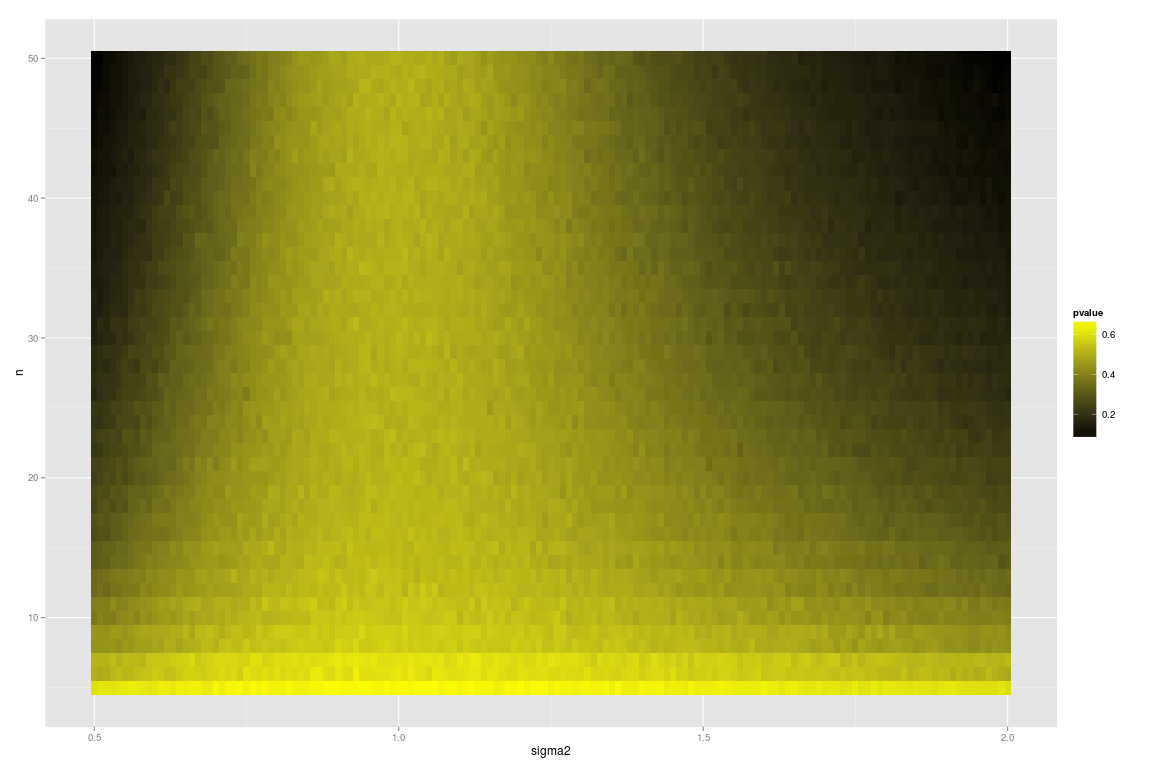
\includegraphics[width=300pt]{wm_pvalue.png}
  \caption{Зависимость достигаемого уровня значимости от значений параметров усредненного по 1000 повторений эксперимента для WM-критерия.}
\end{figure}

\begin{figure}[h]
  \centering
  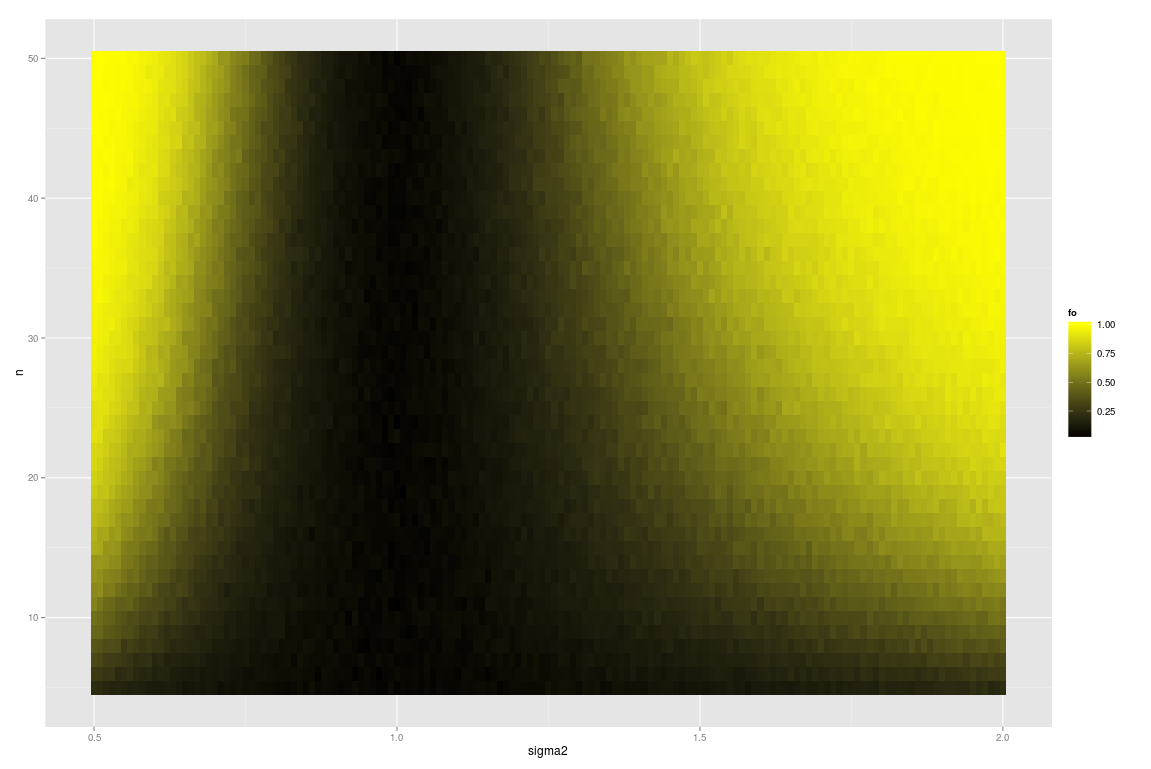
\includegraphics[width=300pt]{f_fo.png}
  \caption{Зависимость эмпирической оценки мощности от значений параметров для критерия Фишера.}
\end{figure}

\begin{figure}[h]
  \centering
  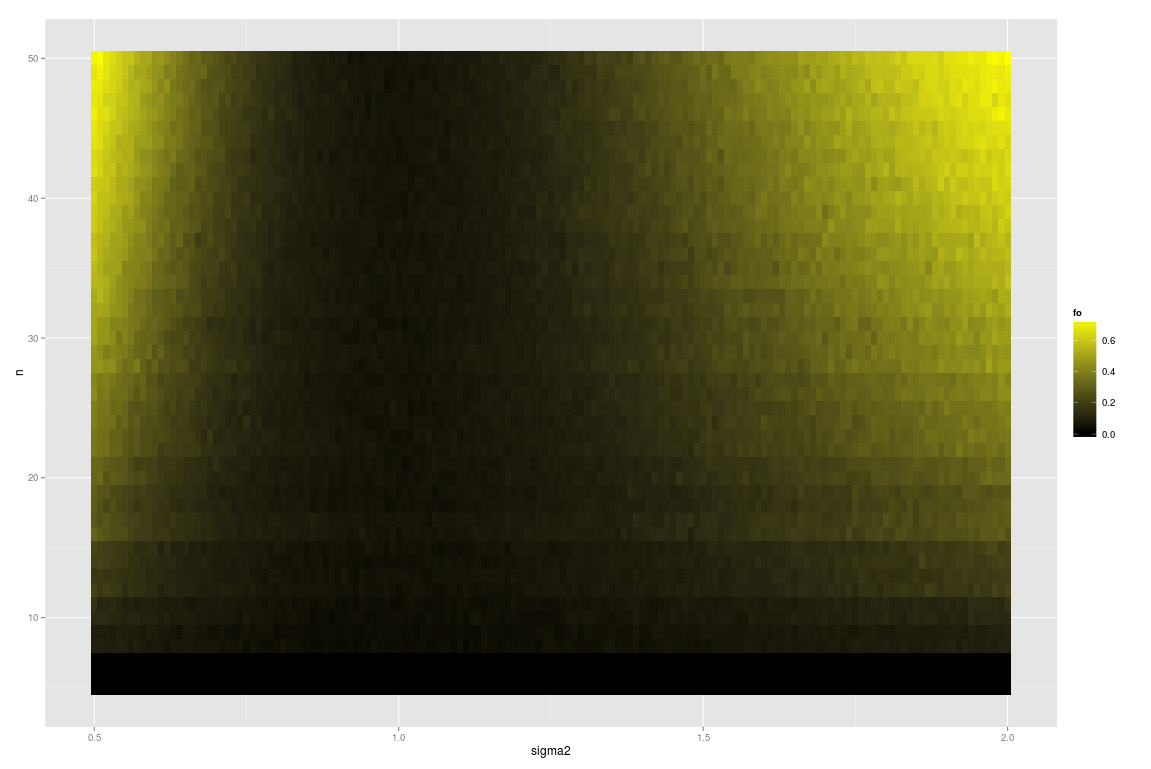
\includegraphics[width=300pt]{wm_fo.png}
  \caption{Зависимость эмпирической оценки мощности от значений параметров для WM-критерия.}
\end{figure}

\begin{figure}[h]
  \centering
  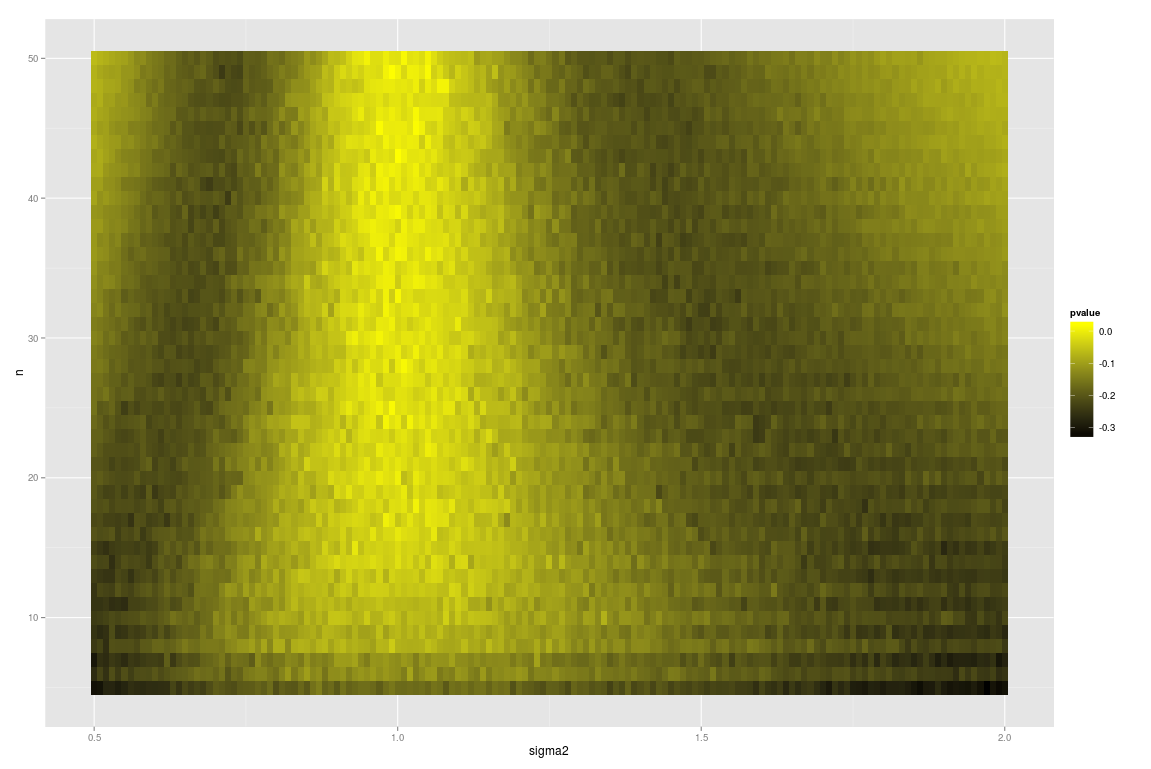
\includegraphics[width=300pt]{diff_pvalue.png}
  \caption{Зависимость достигаемых уровней значимости от значений параметров.}
\end{figure}

\begin{figure}[h]
  \centering
  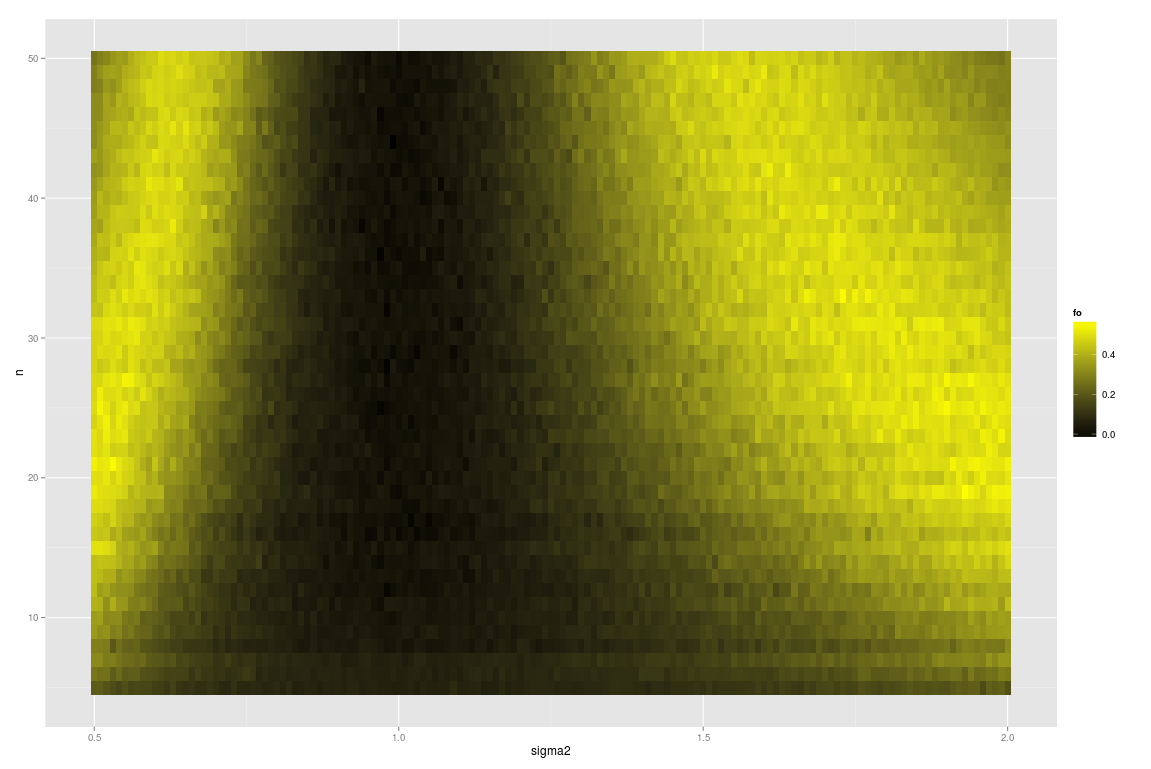
\includegraphics[width=300pt]{diff_fo.png}
  \caption{Зависимость разности эмпирических оценок мощности от значений параметров.}
\end{figure}


\end{document}
